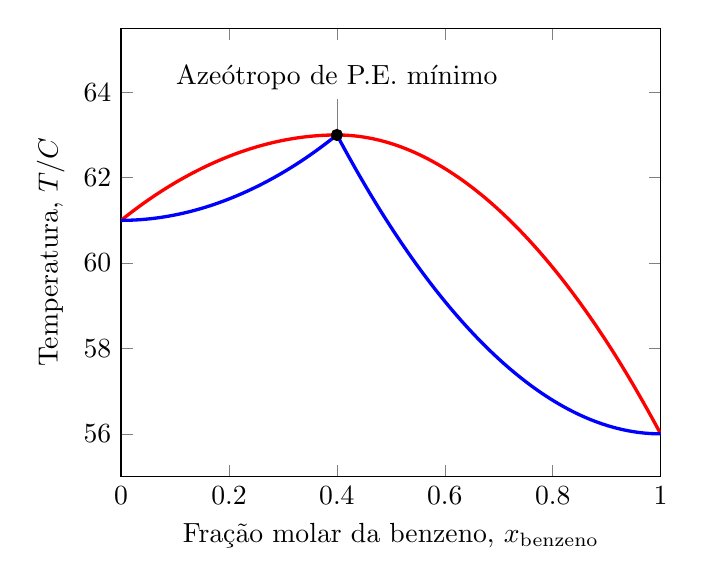
\begin{tikzpicture}
\begin{axis}
    [
        grid = minor,
        xlabel = {Fração molar da benzeno, $x_\mathrm{benzeno}$},
        ylabel = {Temperatura, $T/\unit{\degree C}$},
        xmin = 0, xmax = 1,
        ymin = 55, ymax = 65.5,
    ]    
            
    \draw [draw=red, very thick]
        (axis cs: 0, 61) parabola bend (axis cs: 0.4, 63)
        (axis cs: 1, 56);

    \draw [draw=blue, very thick]
        (axis cs: 0, 61) parabola (axis cs: 0.4, 63);

    \draw [draw=blue, very thick]
        (axis cs: 1, 56) parabola (axis cs: 0.4, 63);

    \addplot [ mark=*, color=black, only marks ] coordinates
        {
            (0.4, 63)
        };

    \node[coordinate, pin={[fill=white, align=left] above:{Azeótropo de P.E. mínimo}}] 
        at (axis cs:0.4, 63) {};
        
\end{axis}
\end{tikzpicture}